\subsection{Ejercicio 4}
\graphicspath{ {img/4} }

\subsubsection{Certificados web}

Los sitios web seleccionados fueron:
\begin{itemize}
    \item \href{https://www.coruna.gal}{coruna.gal}
    \item \href{https://delthia.com}{delthia.com}
    \item \href{https://nap.transportes.gob.es}{nap.transportes.gob.es}
    \item \href{https://www.udc.es}{udc.es}
    \item \href{www.wikipedia.org}{wikipedia.org}
\end{itemize}

\begin{figure}[h]
    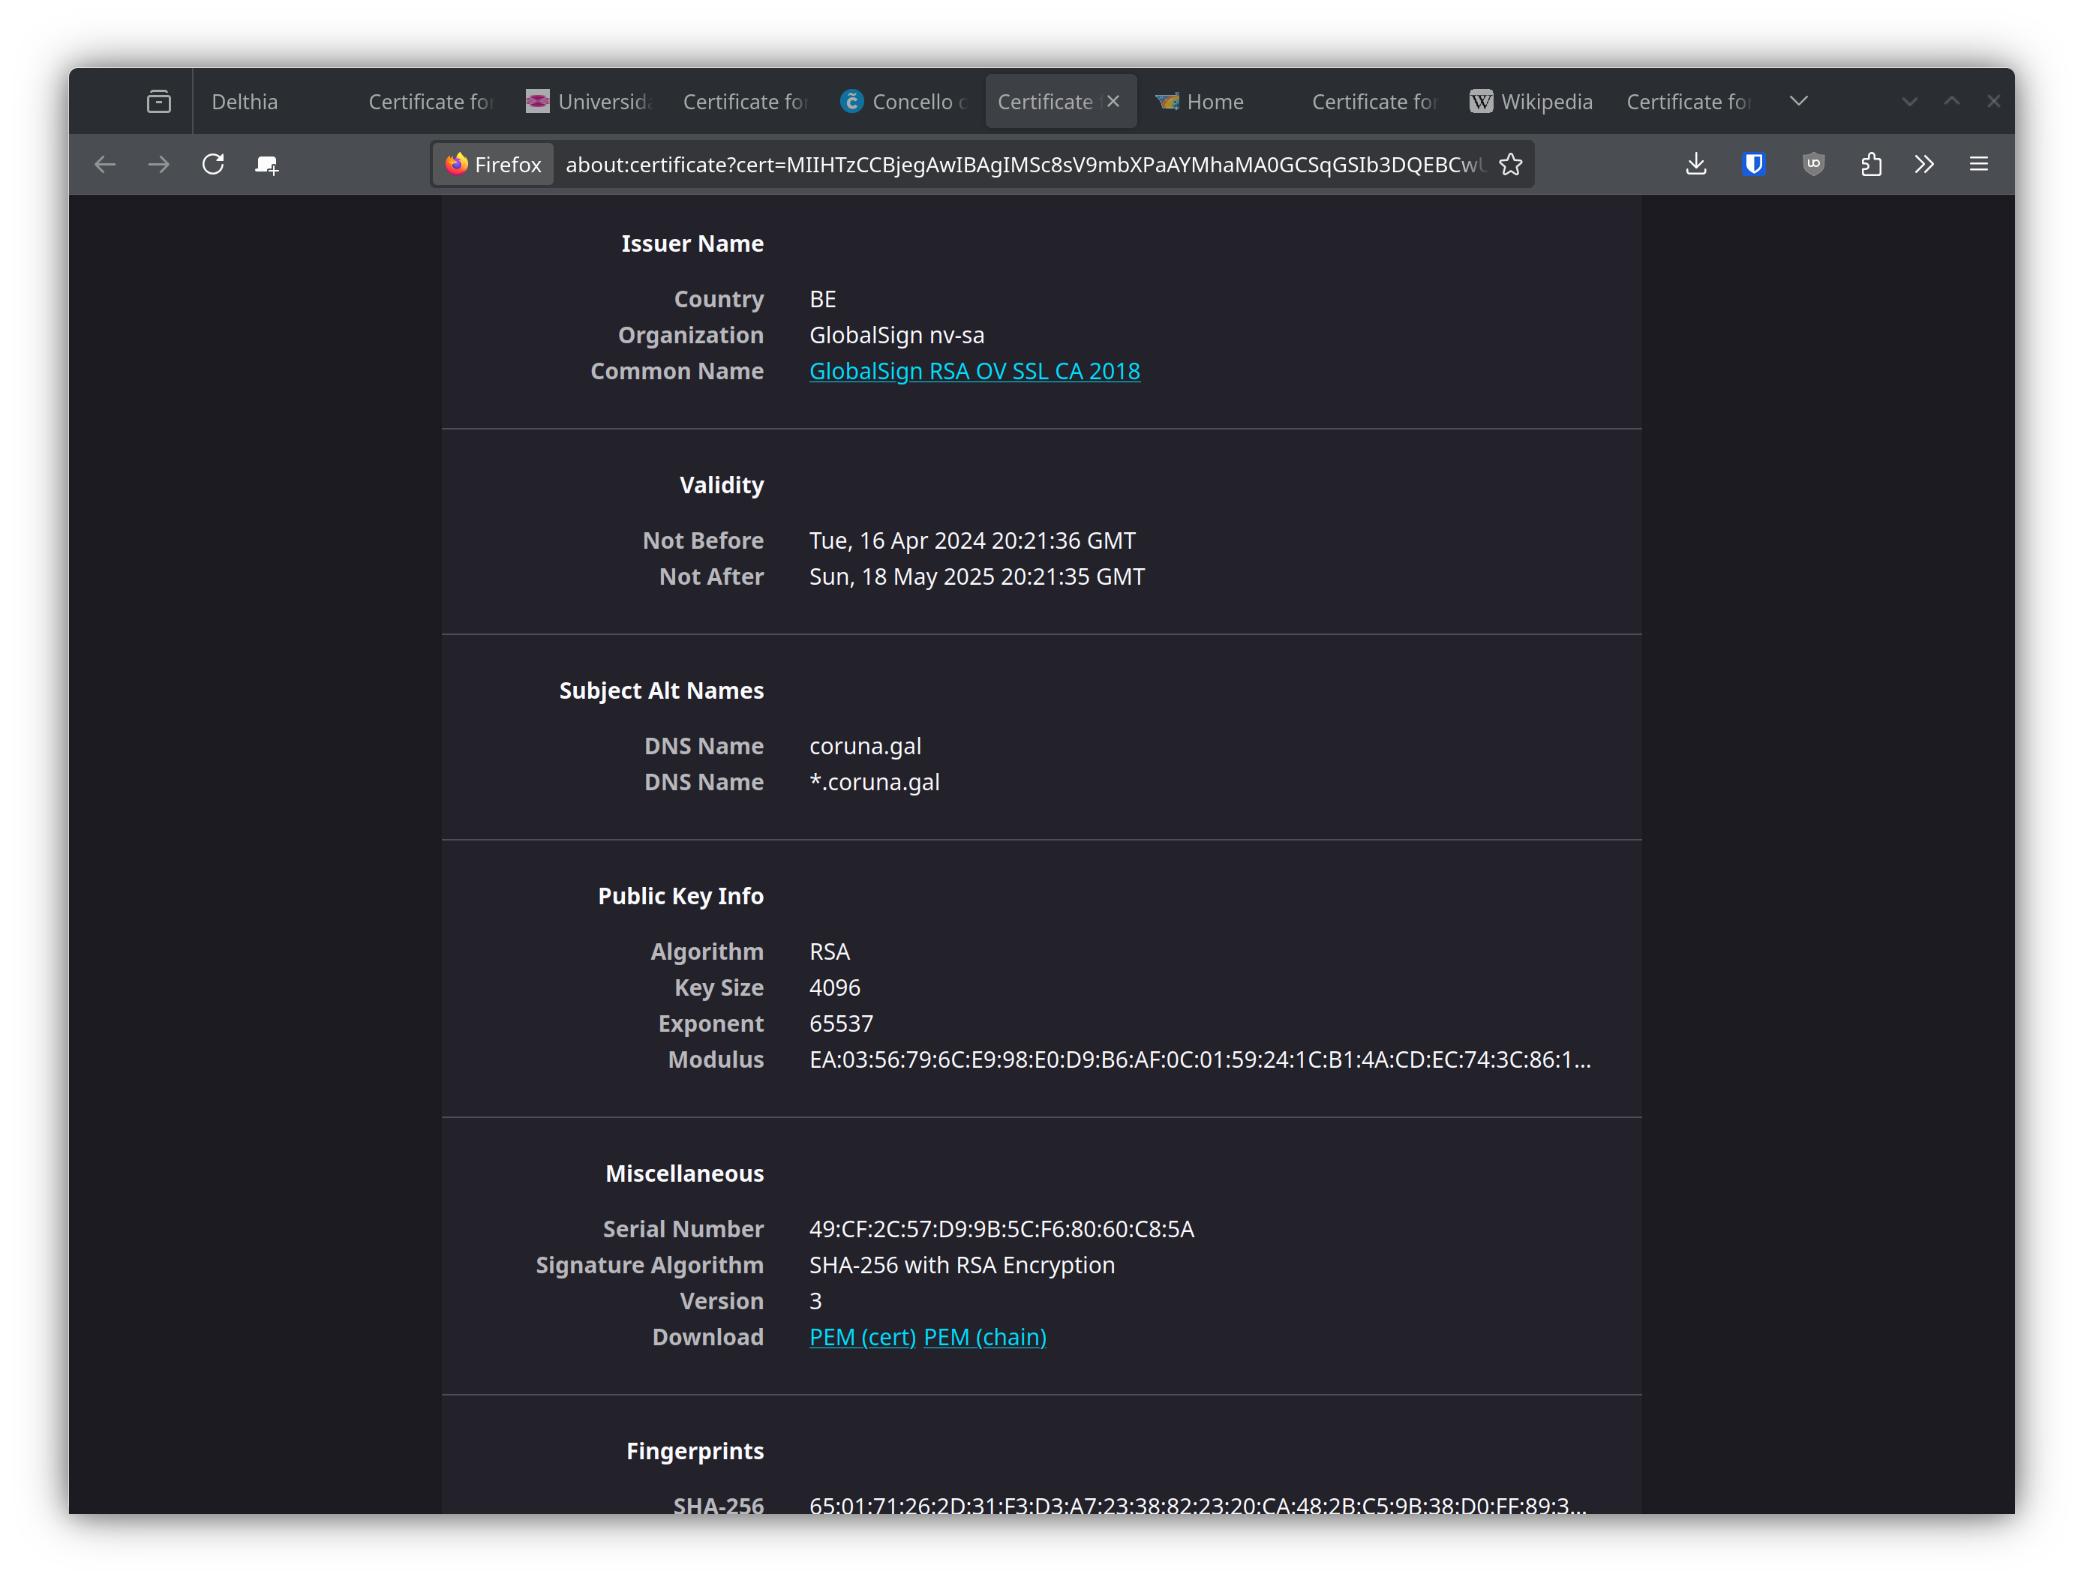
\includegraphics[width=15cm]{cert-coruna.png}
    \caption{Certificado de \url{coruna.gal}}
\end{figure}

\begin{figure}[h]
    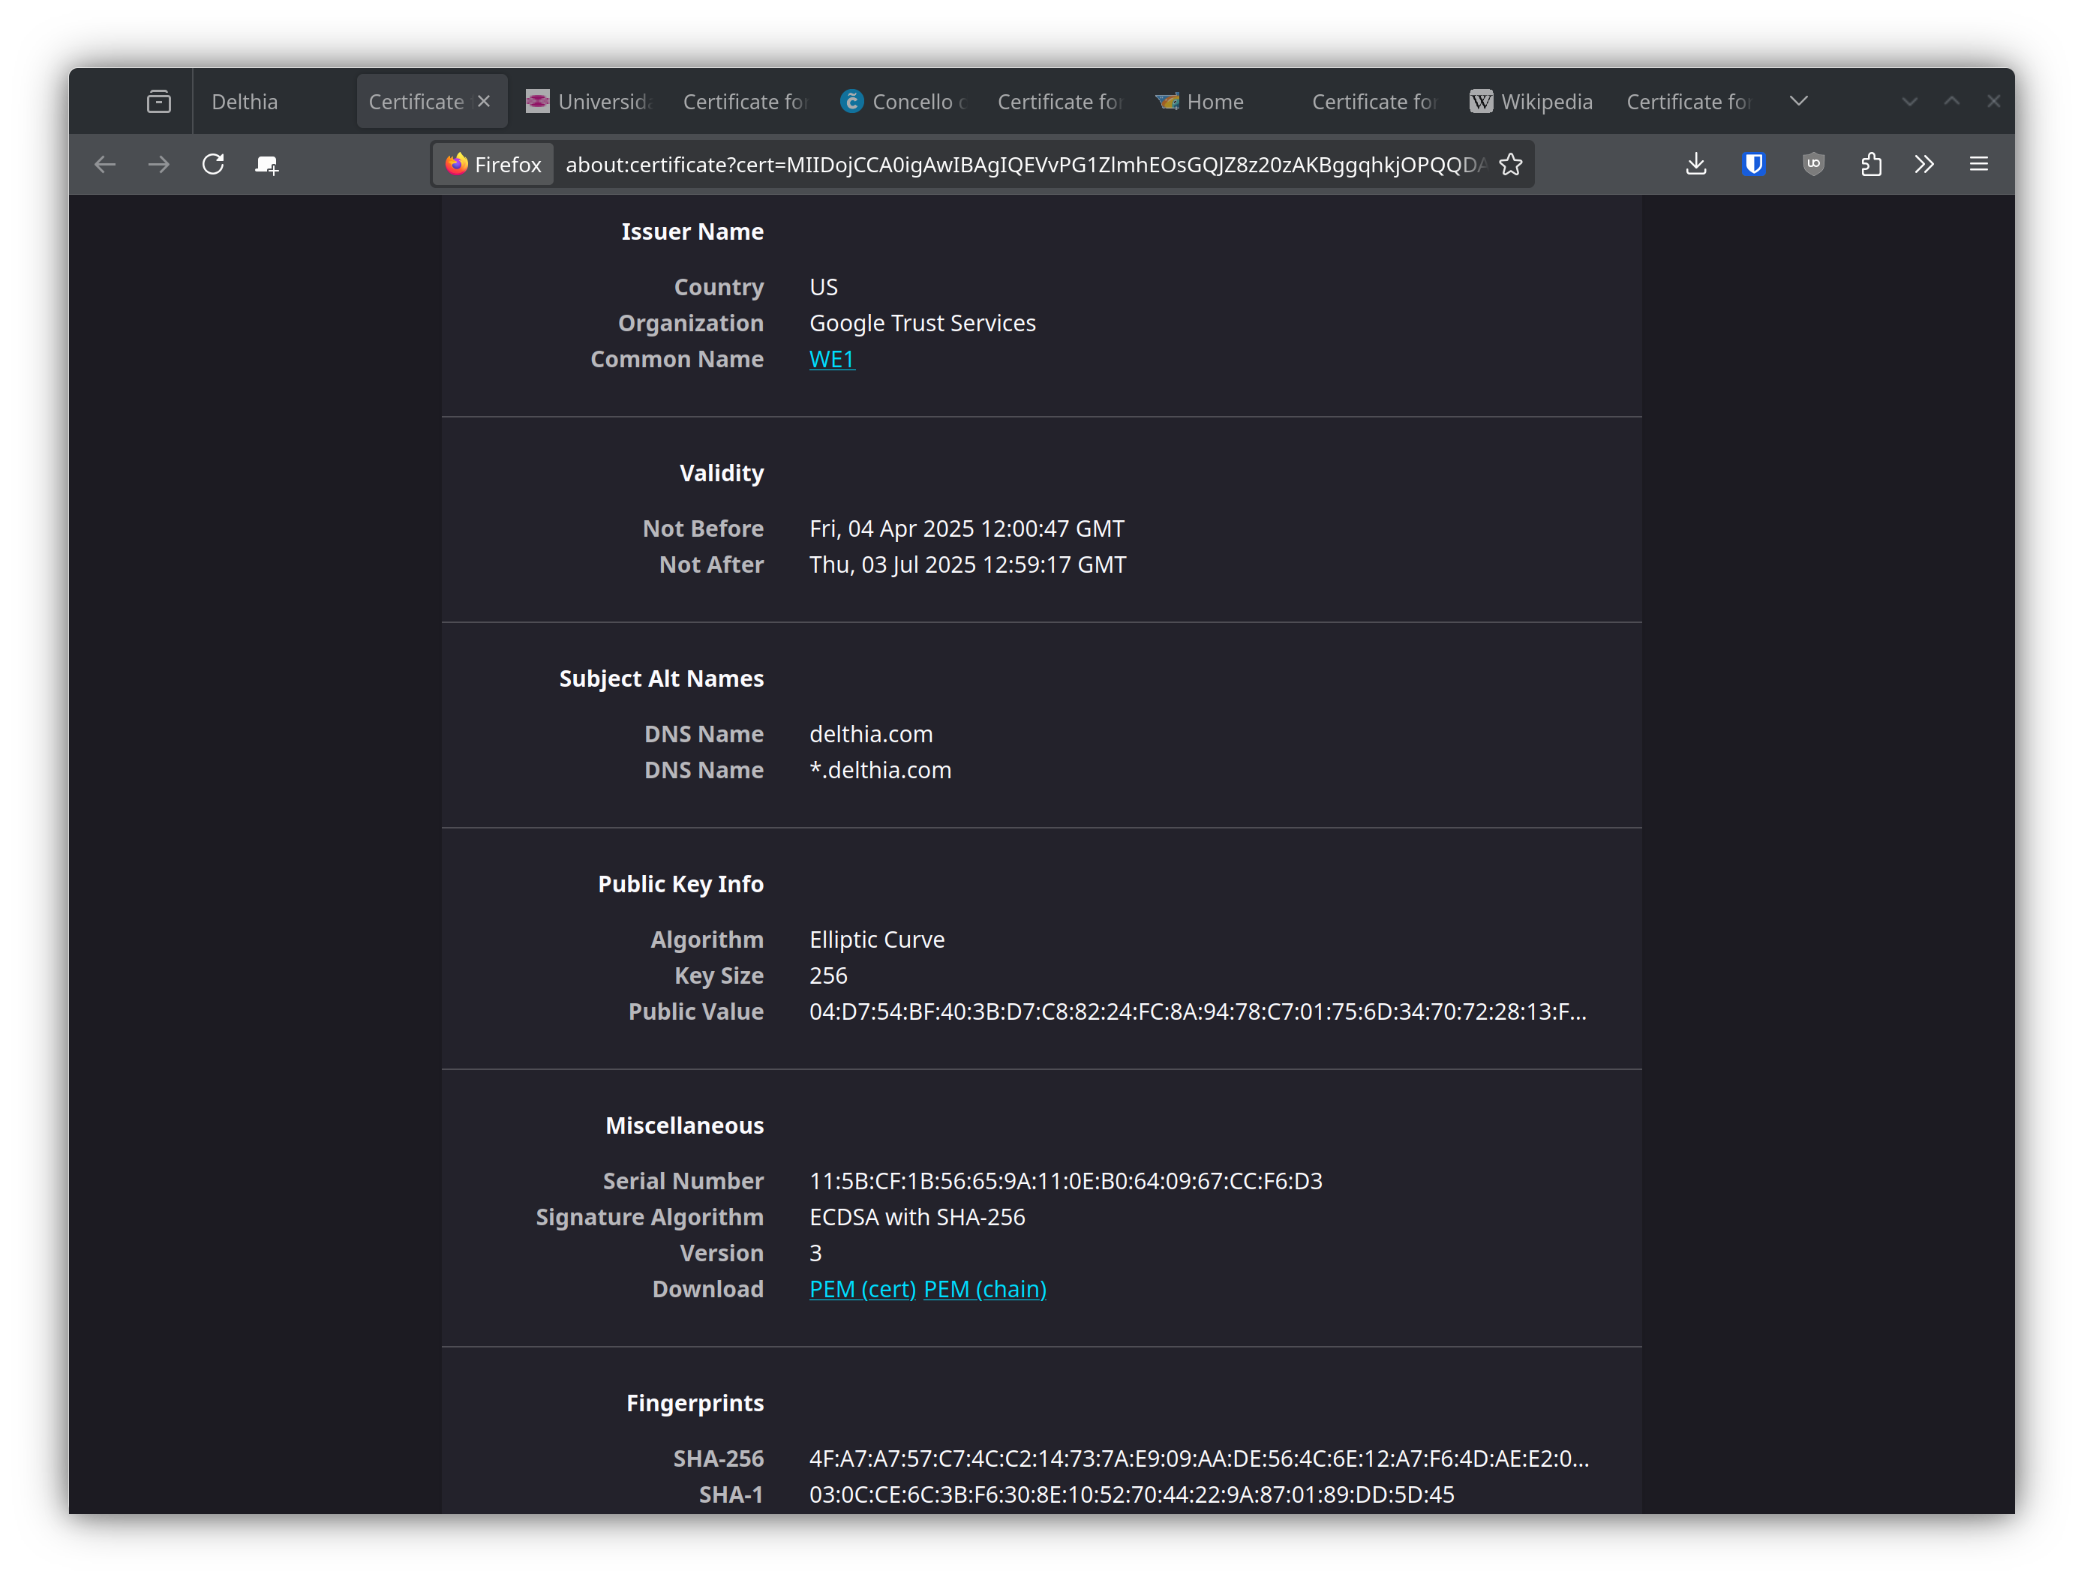
\includegraphics[width=15cm]{cert-delthia.png}
    \caption{Certificado de \url{delthia.com}}
\end{figure}

\begin{figure}[h]
    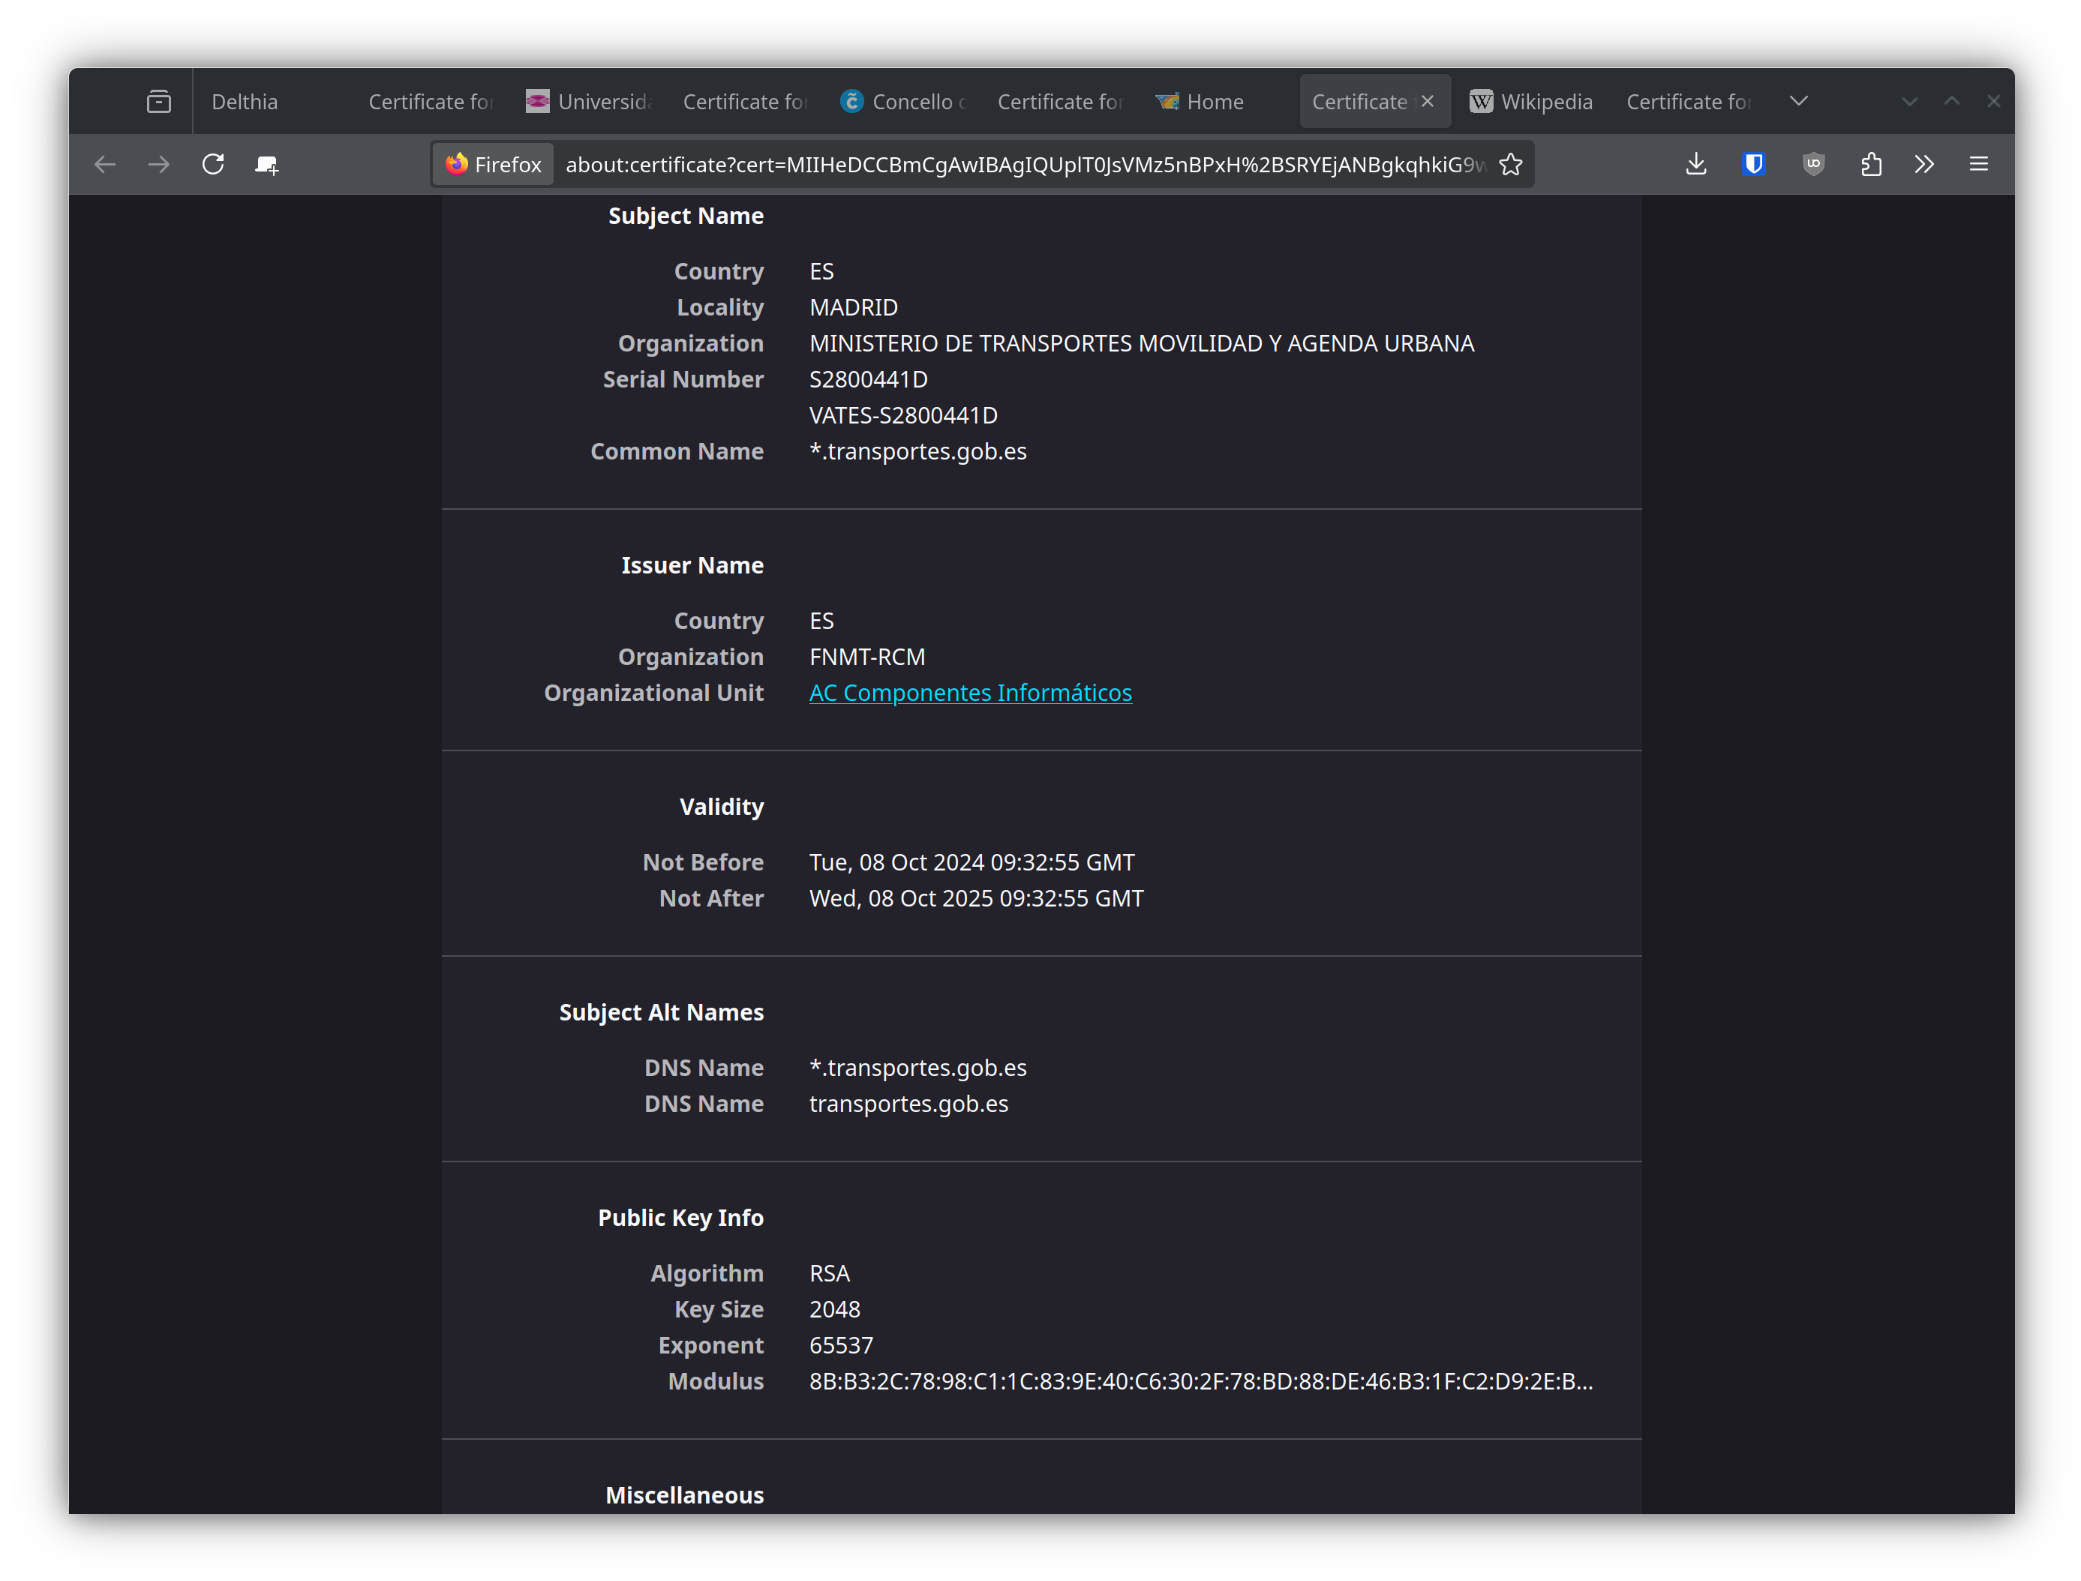
\includegraphics[width=15cm]{cert-transportes.png}
    \caption{Certificado de \url{nap.transportes.gob.es}}
\end{figure}

\begin{figure}[h]
    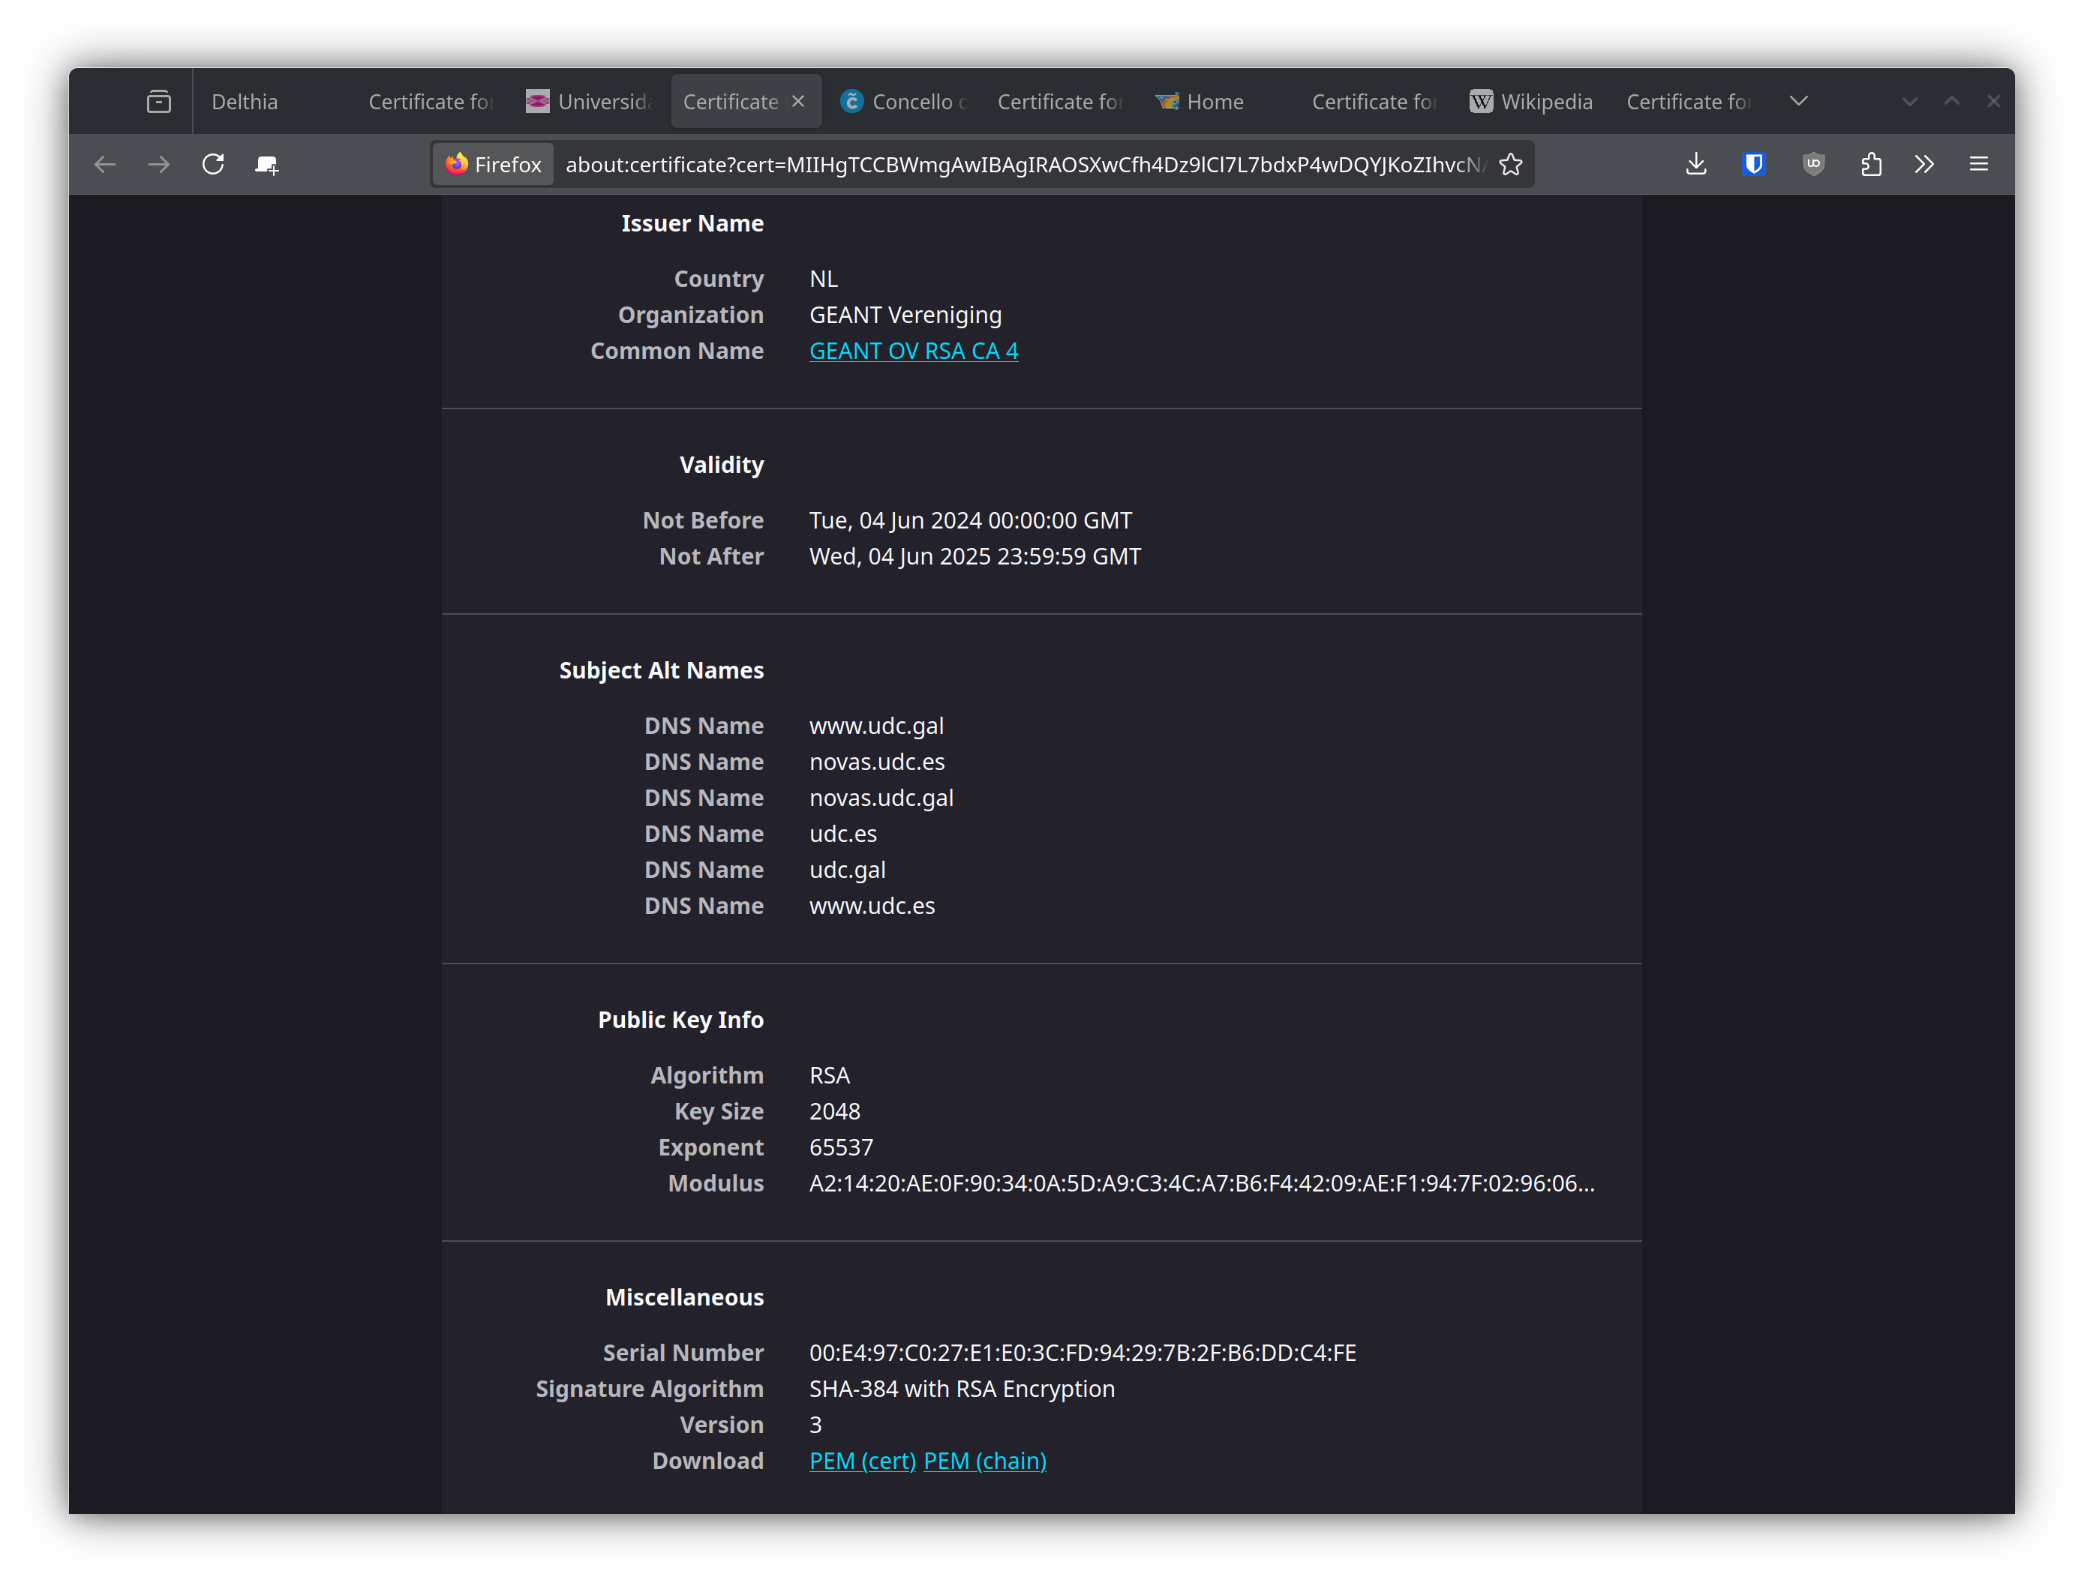
\includegraphics[width=15cm]{cert-udc.png}
    \caption{Certificado de \url{udc.es}}
\end{figure}

\begin{figure}[h]
    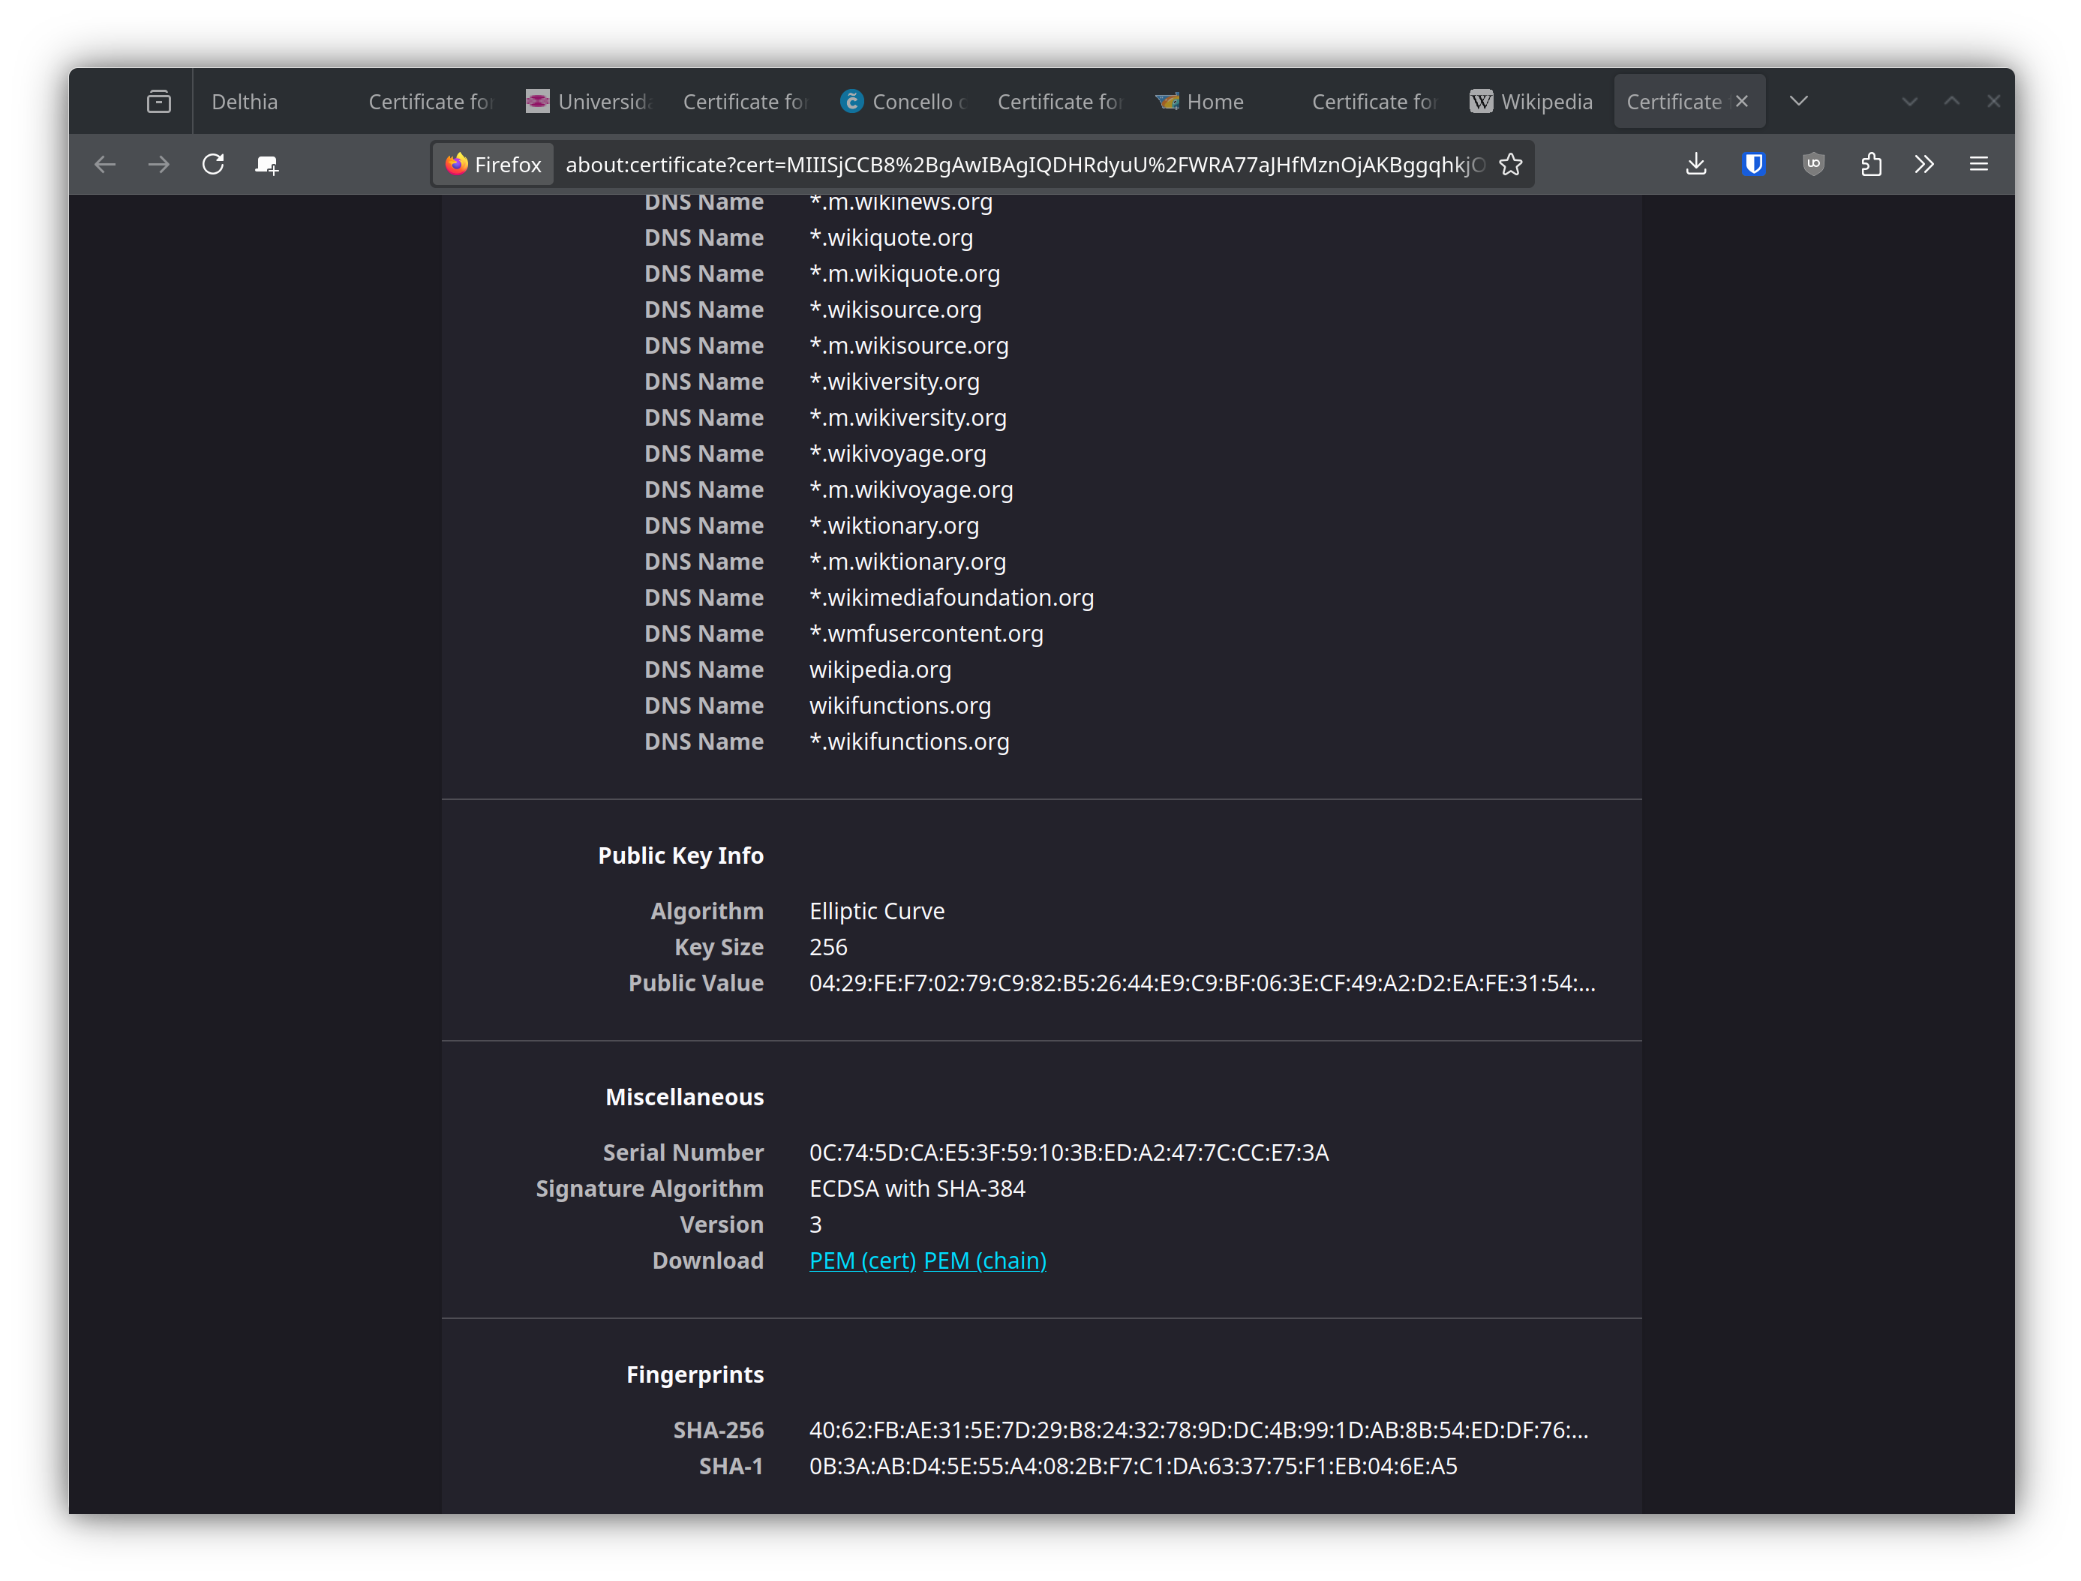
\includegraphics[width=15cm]{cert-wikipedia.png}
    \caption{Certificado de \url{wikipedia.org}}
\end{figure}

\subsubsection{Análisis con openssl}

A continuación se analizan los certificados de \url{coruna.gal} y \url{udc.es}, para lo que utiliza \texttt{OpenSSL} para descargar el certificado y ver los detalles con el comando

\begin{lstlisting}
    openssl s_client -showcerts -servername coruna.gal -connect coruna.gal:443
\end{lstlisting}

Es importante indicar el nombre de deominio del que se desea obtener el certificado, ya que desde un mismo servidor con la misma dirección se pueden servir varios sitios web, dependiendo de la cabecera \texttt{host}.
